\documentclass[12pt,t]{beamer}
\usepackage{graphicx}
\setbeameroption{hide notes}
\setbeamertemplate{note page}[plain]

% get rid of junk
\usetheme{default}
\beamertemplatenavigationsymbolsempty
\hypersetup{pdfpagemode=UseNone} % don't show bookmarks on initial view

% font
\usepackage{fontspec}
\setsansfont{TeX Gyre Heros}
\setbeamerfont{note page}{family*=pplx,size=\footnotesize} % Palatino for notes
% "TeX Gyre Heros can be used as a replacement for Helvetica"
% In Unix, unzip the following into ~/.fonts
% In Mac, unzip it, double-click the .otf files, and install using "FontBook"
%   http://www.gust.org.pl/projects/e-foundry/tex-gyre/heros/qhv2.004otf.zip

% named colors
\definecolor{offwhite}{RGB}{249,242,215}
\definecolor{foreground}{RGB}{255,255,255}
\definecolor{background}{RGB}{24,24,24}
\definecolor{title}{RGB}{107,174,214}
\definecolor{gray}{RGB}{155,155,155}
\definecolor{subtitle}{RGB}{102,255,204}
\definecolor{hilight}{RGB}{102,255,204}
\definecolor{vhilight}{RGB}{255,111,207}
\definecolor{lolight}{RGB}{155,155,155}
\definecolor{hilightlight}{RGB}{102,255,204}
\definecolor{vhilightlight}{RGB}{255,111,207}
%\definecolor{green}{RGB}{125,250,125}

% use those colors
\setbeamercolor{titlelike}{fg=title}
\setbeamercolor{subtitle}{fg=subtitle}
\setbeamercolor{institute}{fg=gray}
\setbeamercolor{normal text}{fg=foreground,bg=background}
\setbeamercolor{item}{fg=foreground} % color of bullets
\setbeamercolor{subitem}{fg=gray}
\setbeamercolor{itemize/enumerate subbody}{fg=gray}
\setbeamertemplate{itemize subitem}{{\textendash}}
\setbeamerfont{itemize/enumerate subbody}{size=\footnotesize}
\setbeamerfont{itemize/enumerate subitem}{size=\footnotesize}

% settings for table of contents
\setbeamercolor{section in toc}{fg=foreground,bg=background}
\setbeamerfont{subsection in toc}{size=\footnotesize}
\setbeamertemplate{section in toc}{{\scriptsize\leavevmode\raise1.35pt\hbox{$\blacktriangleright$}} \inserttocsection}
%\setbeamertemplate{subsection in toc}{\quad{\tiny\leavevmode\raise1.5pt\hbox{$\blacktriangleright$}} \footnotesize\inserttocsubsection\\}
\setbeamertemplate{subsection in toc}{\quad\quad\textendash\enspace\inserttocsubsection\\}

% page number
\setbeamertemplate{footline}{%
    \raisebox{5pt}{\makebox[\paperwidth]{\hfill\makebox[20pt]{\color{gray}
          \scriptsize\insertframenumber}}}\hspace*{5pt}}

% add a bit of space at the top of the notes page
\addtobeamertemplate{note page}{\setlength{\parskip}{12pt}}

% add subsection as frame title when it is empty
\makeatletter
  \CheckCommand*\beamer@checkframetitle{%
    \@ifnextchar\bgroup\beamer@inlineframetitle{}}
  \renewcommand*\beamer@checkframetitle{%
    \global\let\beamer@frametitle\relax\@ifnextchar%
    \bgroup\beamer@inlineframetitle{}}
\makeatother

\addtobeamertemplate{frametitle}{
  \ifx\insertframetitle\empty
      \frametitle{\insertsubsectionhead}
  \else
  \fi
 }{}

% a few macros
\newcommand{\bi}{\begin{itemize}}
\newcommand{\ei}{\end{itemize}}
\newcommand{\ig}{\includegraphics}
\newcommand{\subt}[1]{{\footnotesize \color{subtitle} {#1}}}


% title info
\title{Geometry}
%\subtitle{Part 2}
\author{Tómas Ken Magnússon\\Bjarki Ágúst Guðmundsson}
\institute{\href{http://ru.is/td}{School of Computer Science} \\[2pt] \href{http://ru.is}{Reykjavík University}}
\date{Árangursrík forritun og lausn verkefna}
% \date{\href{http://www.biostat.wisc.edu/~kbroman}{\tt \scriptsize biostat.wisc.edu/{\textasciitilde}kbroman}
% \\[-4pt]
% \href{http://github.com/kbroman}{\tt \scriptsize github.com/kbroman}
% }


% Tikz
\usepackage{tikz}
\usepackage{tkz-euclide}
% \usepackage{intersections}
\usetkzobj{all}
\usetikzlibrary{arrows,shapes,angles,quotes,shapes, calc, decorations}

% Minted
\usepackage{minted}
\usemintedstyle{monokai}
\newminted{cpp}{fontsize=\footnotesize}

% Graph styles
\tikzstyle{vertex}=[circle,fill=black!50,minimum size=15pt,inner sep=0pt, font=\small]
\tikzstyle{selected vertex} = [vertex, fill=red!24]
\tikzstyle{edge} = [draw,thick,-]
\tikzstyle{dedge} = [draw,thick,->]
\tikzstyle{weight} = [font=\scriptsize,pos=0.5]
\tikzstyle{selected edge} = [draw,line width=2pt,-,red!50]
\tikzstyle{ignored edge} = [draw,line width=5pt,-,black!20]


\begin{document}

% title slide
{
    \setbeamertemplate{footline}{} % no page number here
    \frame{
        \titlepage
    }
}

%\AtBeginSection[]
%{
  %\begin{frame}<beamer>{Geometry}
    %\vspace{20pt}
    %\tableofcontents[
      %currentsection,
      %hideallsubsections,
      %%currentsubsection,
      %%hideothersubsections,
      %sectionstyle=show/shaded%,
      %%subsectionstyle=show/shaded/hide
    %]
  %\end{frame}
%}

\begin{frame}<beamer>{Today we're going to cover}
    \vspace{40pt}
    %\tableofcontents[hideallsubsections]
    \bi
      \item Geometry
      \item Computational geometry
    \ei
\end{frame}

\section{Geometry}
\subsection{Points and vectors}

\begin{frame}
  \begin{columns}
    \begin{column}{0.5\textwidth}
      \begin{figure}
        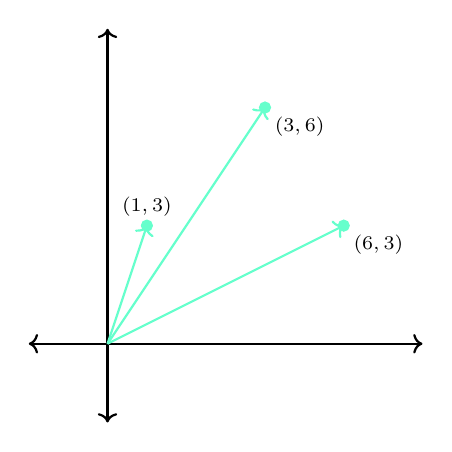
\begin{tikzpicture}
          \draw[step=.5cm, very thin, foreground, opacity=0.2] (0,0) grid (5,5);
          \draw[thick, ->] (1,1) -- (0,1);
          \draw[thick, ->] (1,1) -- (5,1);
          \draw[thick, ->] (1,1) -- (1,0);
          \draw[thick, ->] (1,1) -- (1,5);

          \visible<2->{
            \draw[hilight,fill] (3,4) circle[radius=2pt];
            \draw (3,4) node[anchor=north west] {\scriptsize$(3,6)$};
            \draw[hilight,fill] (4,2.5) circle[radius=2pt];
            \draw (4,2.5) node[anchor=north west] {\scriptsize$(6,3)$};
            \draw[hilight,fill] (1.5,2.5) circle[radius=2pt];
            \draw (1.5,2.5) node[anchor=south] {\scriptsize$(1,3)$};
          }

          \visible<3->{
            \draw[hilight,thick,->] (1,1) -- (3,4);
            \draw[hilight,thick,->] (1,1) -- (4,2.5);
            \draw[hilight,thick,->] (1,1) -- (1.5,2.5);
          }
        \end{tikzpicture}
      \end{figure}
    \end{column}
    \begin{column}{0.5\textwidth}
      \bi
        \onslide<2->
        \item Points are represented by a pair of numbers, $(x,y)$.
        \onslide<3->
        \item Vectors are represented in the same way.
        \item Thinking of points as vectors us to do many things.
      \ei
    \end{column}
  \end{columns}
\end{frame}

\begin{frame}[fragile]
  %Points and vectors can be represented by a pair of numbers, $x$ and $y$.
  \begin{columns}
    \begin{column}{0.5\textwidth}
      \begin{figure}
        \footnotesize
        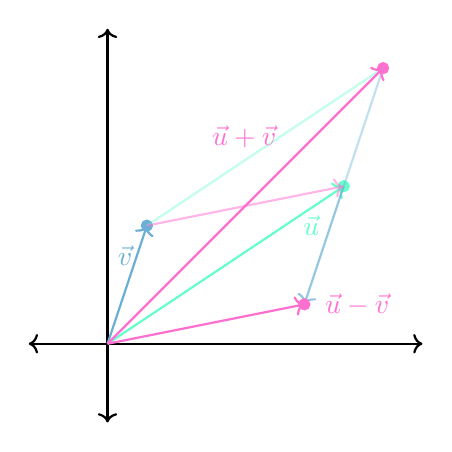
\begin{tikzpicture}
          \draw[step=.5cm, very thin, foreground, opacity=0.2] (0,0) grid (5,5);
          \draw[thick, ->] (1,1) -- (0,1);
          \draw[thick, ->] (1,1) -- (5,1);
          \draw[thick, ->] (1,1) -- (1,0);
          \draw[thick, ->] (1,1) -- (1,5);

          \draw[hilight,fill] (4,3) circle[radius=2pt];
          \draw[title,fill] (1.5,2.5) circle[radius=2pt];

          \draw[hilight,thick,->] (1,1) -- node[right=3pt, near end] {$\vec u$} (4,3);
          \draw[title,thick,->] (1,1) -- node[left=-2pt,near end] {$\vec v$} (1.5,2.5);

          \visible<3>{
            \draw[vhilight,fill] (4.5,4.5) circle[radius=2pt];
            \draw[hilight,thick,opacity=0.4] (1.5,2.5) -- (4.5, 4.5);
            \draw[title,thick,opacity=0.4] (4,3) -- (4.5, 4.5);
            \draw[vhilight,thick,->] (1,1) -- node[left=10pt, near end] {$\vec u + \vec v$} (4.5, 4.5);
          }
          \visible<5>{
            \draw[title,thick,->, opacity=0.7] (4,3) -- (3.5,1.5);
            \draw[vhilight,fill] (3.5,1.5) circle[radius=2pt];
            \draw (3.5,1.5) node[right=4pt] {{\color{vhilight}$\vec u - \vec v$}};
            \draw[vhilight,thick,->] (1,1) --  (3.5, 1.5);
            \draw[vhilight,thick,->, opacity=0.5] (1.5,2.5) -- (4,3);
          }
        \end{tikzpicture}
      \end{figure}
    \end{column}
    \begin{column}{0.5\textwidth}
      %\footnotesize
      \bi
        \onslide<2->
        \item Simplest operation, addition is defined as
          \[
            {\color{title!50}
            \begin{pmatrix}
              x_0 \\
              y_0
            \end{pmatrix}
            }
            +
            {\color{hilight!50}
            \begin{pmatrix}
              x_1 \\
              y_1
            \end{pmatrix}
            }
            =
            {\color{vhilight!50}
            \begin{pmatrix}
              x_0 + x_1 \\
              y_0 + y_1
            \end{pmatrix}
            }
          \]
        \onslide<4->
        \item Subtraction is defined in the same manner
          \[
            {\color{hilight!50}
            \begin{pmatrix}
              x_0 \\
              y_0
            \end{pmatrix}
            }
            -
            {\color{title!50}
            \begin{pmatrix}
              x_1 \\
              y_1
            \end{pmatrix}
            }
            =
            {\color{vhilight!50}
            \begin{pmatrix}
              x_0 - x_1 \\
              y_0 - y_1
            \end{pmatrix}
            }
          \]
      \ei
    \end{column}
  \end{columns}
\end{frame}

\begin{frame}[fragile]
  \begin{minted}{cpp}
struct point {
    double x, y;
    point(double _x, double _y) { 
        x = _x, y = _y;
    }

    point operator+(const point &oth){
        return point(x + oth.x, y + oth.y);
    }

    point operator-(const point &oth){
        return point(x - oth.x, y - oth.y);
    }
};
  \end{minted}
\end{frame}

\begin{frame}[fragile]
  \vspace{20pt}
  \ldots or we could use the \texttt{complex<double>} class.
  \begin{minted}{cpp}
typedef complex<double> point;
  \end{minted}
  \onslide<2->
  \vspace{10pt}
  The \texttt{complex} class in \texttt{C++} and \texttt{Java} has methods defined for
  \bi
    \item Addition
    \item Subtraction
    \item Multiplication by a scalar
    \item Length
    \item Trigonometric functions
  \ei
\end{frame}

\begin{frame}[fragile]
  \vspace{20pt}
  Complex numbers have the real part and the imaginary part. Can be thought of
  as vectors or points on the complex plane.
  \bi
    \onslide<2->
    \item \mintinline{cpp}{double real(p)} returns the real part, or in our case, the $x$ value
      of \mintinline{cpp}{p}
    \onslide<3->
    \item \mintinline{cpp}{double imag(p)} returns the imaginary part, $y$ value of \mintinline{cpp}{p}.
    \onslide<4->
    \item \mintinline{cpp}{double abs(p)} returns the absolute value of the complex number, the
      length of the vector.
    \onslide<5->
    \item \mintinline{cpp}{double sin(p)}, \mintinline{cpp}{double cos(p)}, \mintinline{cpp}{double tan(p)}, trigonometric
      functions.
  \ei
\end{frame}

\subsection{Lines and line segments}
\begin{frame}[fragile]
  \begin{columns}
    \begin{column}{0.5\textwidth}
      \begin{figure}
        \footnotesize
        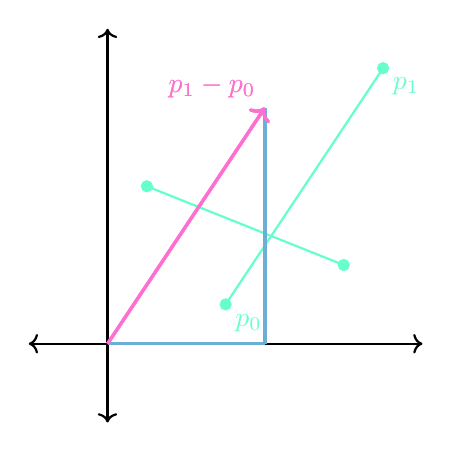
\begin{tikzpicture}
          \draw[step=.5cm, very thin, foreground, opacity=0.2] (0,0) grid (5,5);
          \draw[thick, ->] (1,1) -- (0,1);
          \draw[thick, ->] (1,1) -- (5,1);
          \draw[thick, ->] (1,1) -- (1,0);
          \draw[thick, ->] (1,1) -- (1,5);
          \visible<1>{
            \draw[hilight,fill] (1.5,3) circle[radius=2pt];
            %\draw (1.5,3) node[anchor=south] {\scriptsize$(1,4)$};
            \draw[hilight,fill] (4,2) circle[radius=2pt];
            %\draw (4,2) node[anchor=north west] {\scriptsize$(6,2)$};
            \draw[hilight,thick] (1.5,3) -- (4,2);
          }

          \visible<1-2>{
            \draw[hilight,fill] (2.5,1.5) circle[radius=2pt];
            \draw[hilight,fill] (4.5,4.5) circle[radius=2pt];
            \draw[hilight,thick] (2.5,1.5) -- (4.5,4.5);
          }

          \visible<2>{
            \draw (2.5,1.5) node[anchor=north west] {{\color{hilight}$p_0$}};
            \draw (4.5,4.5) node[anchor=north west] {{\color{hilight}$p_1$}};
            \draw[vhilight,very thick,->] (1,1) -- (3,4);
            \draw (3,4) node[anchor=south east] {{\color{vhilight}$p_1 - p_0$}};
          }

          \visible<3>{
            \draw[title,very thick] (1,1) -- (3,1);
            \draw[title,very thick] (3,1) -- (3,4);
            \draw[vhilight,very thick,->] (1,1) -- (3,4);
            \draw (3,4) node[anchor=south east] {{\color{vhilight}$p_1 - p_0$}};
          }
        \end{tikzpicture}
      \end{figure}
    \end{column}
    \begin{column}{0.55\textwidth}
      \bi
        \item Line segments are represented by a pair of points, $((x_0,y_0), (x_1,y_1))$.
        \onslide<2->
        \item Distance between two points is the length of the line segment or vector between the points.
          \onslide<3->
          \begin{align*}
            d((x_0, &y_0), (x_1,y_1)) \\
            &= \lvert(x_1 - x_0, y_1 - y_0)\rvert \\
            &= \sqrt{(x_1 - x_0)^2 + (y_1 - y_0)^2}
          \end{align*}
      \ei
    \end{column}
  \end{columns}
\end{frame}

\begin{frame}[fragile]
  \vspace{30pt}
  \begin{minted}{cpp}
struct point {
    ...
    double distance(point oth = point(0,0)) const {
        return sqrt(pow(x - oth.x, 2.0)
                  + pow(y - oth.y, 2.0));
    }
    ...
}
  \end{minted}
  \onslide<2->
  \vspace{20pt}
  Or use the \texttt{abs} function with \texttt{complex<double>}.
\end{frame}

\begin{frame}[fragile]
  \begin{columns}
    \begin{column}{0.5\textwidth}
      \begin{figure}
        \footnotesize
        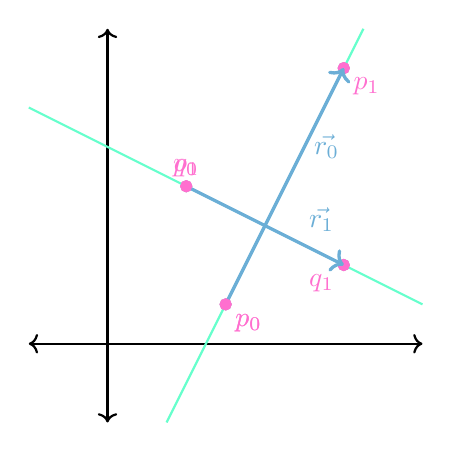
\begin{tikzpicture}
          \draw[step=.5cm, very thin, foreground, opacity=0.2] (0,0) grid (5,5);
          \draw[thick, ->] (1,1) -- (0,1);
          \draw[thick, ->] (1,1) -- (5,1);
          \draw[thick, ->] (1,1) -- (1,0);
          \draw[thick, ->] (1,1) -- (1,5);

          \draw[hilight,fill] (2,3) circle[radius=2pt];
          \draw[hilight,fill] (4,2) circle[radius=2pt];
          \draw[hilight,thick] (2,3) -- (4,2);

          \draw[hilight,fill] (2.5,1.5) circle[radius=2pt];
          \draw[hilight,fill] (4,4.5) circle[radius=2pt];
          \draw[hilight,thick] (2.5,1.5) -- (4,4.5);

          \visible<2>{
            \draw (4,2) node[anchor=north east] {{\color{vhilight}$q_1$}};
            \draw (4,4.5) node[anchor=north west] {{\color{vhilight}$p_1$}};
            \draw (2,3) node[anchor=south] {{\color{vhilight}$q_0$}};
            \draw (2.5,1.5) node[anchor=north west] {{\color{vhilight}$p_0$}};
          }
          \visible<2->{
            \draw[hilight,thick] (5,1.5) -- (0,4);
            \draw[hilight,thick] (1.75,0) -- (4.25,5);

            \draw[vhilight,fill] (2,3) circle[radius=2pt];
            \draw[vhilight,fill] (4,2) circle[radius=2pt];

            \draw[vhilight,fill] (2.5,1.5) circle[radius=2pt];
            \draw[vhilight,fill] (4,4.5) circle[radius=2pt];
          }

          \visible<3->{
            \draw[vhilight,fill] (4,2) circle[radius=2pt];
            \draw[title,very thick,->] (2,3) -- (4,2);
            \draw[vhilight,fill] (2,3) circle[radius=2pt];

            \draw[vhilight,fill] (4,4.5) circle[radius=2pt];
            \draw[title,very thick,->] (2.5,1.5) -- (4,4.5);
            \draw[vhilight,fill] (2.5,1.5) circle[radius=2pt];

            \draw (2,3) node[anchor=south] {{\color{vhilight}$p_1$}};
            \draw (2.5,1.5) node[anchor=north west] {{\color{vhilight}$p_0$}};

            \draw (3.5,3.5) node[anchor=west] {{\color{title}$\vec{r_0}$}};
            \draw (4,2.3) node[anchor=south east] {{\color{title}$\vec{r_1}$}};
          }
        \end{tikzpicture}
      \end{figure}
    \end{column}
    \begin{column}{0.6\textwidth}
      %\vspace{20pt}
      \bi
        \item Line representation same as line segments.
        \onslide<2->
        \item Treat them as lines passing through the two points.
        \onslide<3->
        \item Or as a point and a direction vector.
          \[
            {\color{vhilight!70}p} + {\color{hilight!70}t} \cdot {\color{title!80}\vec{r}}
          \]
        \onslide<4->
        \vspace{-10pt}
        \item Either way
          \begin{minted}{cpp}
pair<point,point>
          \end{minted}
      \ei
    \end{column}
  \end{columns}
\end{frame}

\subsection{Circles}
\begin{frame}[fragile]
  \begin{columns}
    \begin{column}{0.5\textwidth}
      \begin{figure}
        \footnotesize
        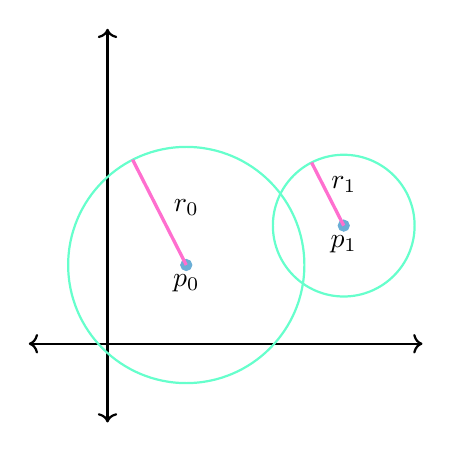
\begin{tikzpicture}
          \draw[step=.5cm, very thin, foreground, opacity=0.2] (0,0) grid (5,5);
          \draw[thick, ->] (1,1) -- (0,1);
          \draw[thick, ->] (1,1) -- (5,1);
          \draw[thick, ->] (1,1) -- (1,0);
          \draw[thick, ->] (1,1) -- (1,5);

          \draw[hilight,thick] (2,2) circle[radius=1.5cm];
          \draw[hilight,thick] (4,2.5) circle[radius=0.9cm];
          %\draw (3,4) node[anchor=north west] {\scriptsize$(3,6)$};

          \visible<2->{
            \draw[title,fill] (2,2) circle[radius=2pt];
            \draw (2,2) node[anchor=north] {$p_0$};
            \draw[title,fill] (4,2.5) circle[radius=2pt];
            \draw (4,2.5) node[anchor=north] {$p_1$};
          }

          \visible<3->{
            %\draw (2,2) -- (0,10);
            \draw[vhilight,very thick] (2,2) --  +(117:1.5cm) ;
            \draw[vhilight,very thick] (4,2.5) --  +(117:0.9cm) ;
            \draw (2,2.5) node[anchor=south] {$r_0$};
            \draw (4,2.8) node[anchor=south] {$r_1$};
          }
        \end{tikzpicture}
      \end{figure}
    \end{column}
    \begin{column}{0.5\textwidth}
      \vspace{20pt}
      \bi
        \item Circles are very easy to represent.
        \onslide<2->
        \item Center point ${\color{title!80}p = (x,y)}$.
        \onslide<3->
        \item And the radius ${\color{vhilight!70}r}$.
        \onslide<4->
        \begin{minted}{cpp}
pair<point,double>
        \end{minted}
      \ei
    \end{column}
  \end{columns}
\end{frame}

\subsection{Dot product}
\begin{frame}
  \vspace{20pt}
  Given two vectors 
  \[
    \vec{u} = \begin{pmatrix} x_0 \\ y_0 \end{pmatrix} \quad\quad
    \vec{v} = \begin{pmatrix} x_1 \\ y_1 \end{pmatrix}
  \]
  the dot product of $\vec{u}$ and $\vec{v}$ is defined as 
  \[
    \begin{pmatrix} x_0 \\ y_0 \end{pmatrix} \cdot
    \begin{pmatrix} x_1 \\ y_1 \end{pmatrix} = 
    x_0 \cdot x_1 + y_0 \cdot y_1
  \]
  \onslide<2->
  Which in geometric terms is
  \[
    \vec{u} \cdot \vec{v} = 
    \lvert \vec{u} \rvert \lvert \vec{v} \rvert \cos \theta
  \]
\end{frame}

%\begin{frame}
  %\begin{columns}
    %\begin{column}{0.4\textwidth}
      %\vspace{20pt}
      %\begin{figure}
        %\begin{tikzpicture}
          %\draw[fill=title!50] (0,0) -- (40:.75cm) arc (40:0:.75cm);
          %\draw[->,thick,hilight] (0,0) -- node[near end, below] {$\vec u$} (0:4cm);
          %\draw[->,thick,vhilight] (0,0) -- node[near end, left=4pt] {$\vec v$} (40:3.2cm);
          %\draw(22:0.5cm) node {\color{background}$\theta$};

          %\visible<2->{
            %\draw[dashed] (40:3.2cm) -- (0:2.45134221cm);
            %\draw[title,thick,->] (0,0) -- node[below] {$\vec{v}_{\vec{u}}$} (0:2.45134221cm);
          %}
        %\end{tikzpicture}
      %\end{figure}
    %\end{column}
    %\begin{column}{0.6\textwidth}
      %\bi
        %\item Allows us to calculate the angle between $\vec u$ and $\vec v$.
          %\[
            %\theta = \arccos\left(\frac{\vec{u} \cdot \vec{v}}{\lvert \vec u \rvert \lvert \vec v \rvert}\right)
          %\]
        %\onslide<2->
        %\item And the projection of $\vec v$ onto $\vec u$.
          %\[
            %\vec{v}_{\vec{u}} = \left(\frac{\vec{u}\cdot\vec{v}}{\lvert u \rvert}\right) \vec{u}
          %\]
      %\ei
    %\end{column}
  %\end{columns}
%\end{frame}

\begin{frame}
  \begin{columns}
    \begin{column}{0.4\textwidth}
      \vspace{20pt}
      \begin{figure}
        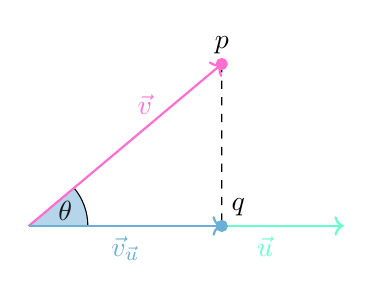
\begin{tikzpicture}
          \draw[fill=title!50] (0,0) -- (40:.75cm) arc (40:0:.75cm);
          \draw[->,thick,hilight] (0,0) -- node[near end, below] {$\vec u$} (0:4cm);
          \draw[->,thick,vhilight] (0,0) -- node[near end, left=4pt] {$\vec v$} (40:3.2cm);
          \draw(22:0.5cm) node {\color{background}$\theta$};

          \visible<2->{
            \draw[dashed] (40:3.2cm) -- (0:2.45134221cm);
            \draw[title,thick,->] (0,0) -- node[below] {$\vec{v}_{\vec{u}}$} (0:2.45134221cm);
          }

          \visible<3->{
            \draw (40:3.2cm) node[above] {$p$};
            \draw[fill,vhilight] (40:3.2cm) circle[radius=2pt];
            \draw (0:2.45134221cm) node[above right] {$q$};
            \draw[fill,title] (0:2.45134221cm) circle[radius=2pt];
          }
        \end{tikzpicture}
      \end{figure}
    \end{column}
    \begin{column}{0.6\textwidth}
      \bi
        \only<1-2>{
          \item Allows us to calculate the angle between $\vec u$ and $\vec v$.
            \[
              \theta = \arccos\left(\frac{\vec{u} \cdot \vec{v}}{\lvert \vec u \rvert \lvert \vec v \rvert}\right)
            \]
        }
        \only<2>{
          \item And the projection of $\vec v$ onto $\vec u$.
            \[
              \vec{v}_{\vec{u}} = \left(\frac{\vec{u}\cdot\vec{v}}{\lvert u \rvert}\right) \vec{u}
            \]
        }
        \only<3->{
          \vspace{20pt}
          \item The closest point on $\vec{u}$ to $p$ is $q$.
        }
        \only<4->{
          \item The distance from $p$ to $\vec{u}$ is the distance from $p$ to $q$.
        }
        \only<5->{
          \item Unless $q$ is outside $\vec{u}$, then the closest point is either of the endpoints.
        }
      \ei
    \end{column}
  \end{columns}
\end{frame}

\begin{frame}[fragile]
  \vspace{20pt}
  Rest of the code will use the \texttt{complex} class.
  \footnotesize
  \begin{minted}{cpp}
#define P(p) const point &p
#define L(p0, p1) P(p0), P(p1)
double dot(P(a), P(b)) { 
    return real(a) * real(b) + imag(a) * imag(b);
}
double angle(P(a), P(b), P(c)) {
    return acos(dot(b - a, c - b) / abs(b - a) / abs(c - b)); 
}
point closest_point(L(a, b), P(c), bool segment = false) {
    if (segment) {
        if (dot(b - a, c - b) > 0) return b;
        if (dot(a - b, c - a) > 0) return a;
    }
    double t = dot(c - a, b - a) / norm(b - a);
    return a + t * (b - a);
}
  \end{minted}
\end{frame}
\subsection{Cross product}
\begin{frame}
  \vspace{20pt}
  Given two vectors
  \[
    \vec{u} = \begin{pmatrix} x_0 \\ y_0 \end{pmatrix} \quad\quad
    \vec{v} = \begin{pmatrix} x_1 \\ y_1 \end{pmatrix}
  \]
  the cross product of $\vec{u}$ and $\vec{v}$ is defined as 
  \[
    \left\lvert \begin{pmatrix} x_0 \\ y_0 \end{pmatrix} \times
    \begin{pmatrix} x_1 \\ y_1 \end{pmatrix}\right\rvert  = 
    x_0\cdot y_1 - y_0 \cdot x_1
  \]
  \onslide<2->
  Which in geometric terms is
  \[
    \lvert \vec{u} \times \vec{v} \vert = 
    \lvert \vec{u} \rvert \lvert \vec{v} \rvert \sin \theta
  \]
\end{frame}

\begin{frame}
  \begin{columns}
    \begin{column}{0.4\textwidth}
      \vspace{20pt}
      \begin{figure}
        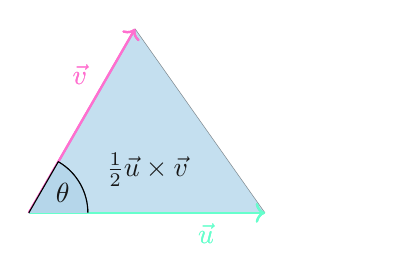
\begin{tikzpicture}
          \coordinate (A) at (0,0);
          \coordinate (B) at (0:3cm);
          \coordinate (D) at (60:2.7cm);
          \coordinate (C) at ($ (B) + (D) $);

          \tkzDrawPolygon[color=foreground](A,B,C,D);
          \draw[fill=title!50] (0,0) -- (60:.75cm) arc (60:0:.75cm);
          \draw[->,thick,hilight] (0,0) -- node[near end, below] {$\vec u$} (B);
          \draw[->,thick,vhilight] (0,0) -- node[near end, left=4pt] {$\vec v$} (D);
          \draw(30:0.5cm) node {\color{background}$\theta$};

          \visible<2->{
            %\draw[title,thick,->] (0,0) -- node[below] {$\vec{v}_{\vec{u}}$} (0:2.45134221cm);
            \tkzDrawPolygon[fill=title,opacity=0.4](A,B,D);
            \draw (20:1.6cm) node {\color{background}$\frac{1}{2}\lvert \vec{u} \times \vec{v} \rvert$};
            \draw[->,thick,hilight] (0,0) -- node[near end, below] {$\vec u$} (B);
            \draw[->,thick,vhilight] (0,0) -- node[near end, left=4pt] {$\vec v$} (D);
            \draw[fill=title!50] (0,0) -- (60:.75cm) arc (60:0:.75cm);
            \draw(30:0.5cm) node {\color{background}$\theta$};
          }
        \end{tikzpicture}
      \end{figure}
    \end{column}
    \begin{column}{0.6\textwidth}
      \bi
        \item Allows us to calculate the area of the triangle formed by $\vec u$ and $\vec v$.
          \[
            \frac{\lvert \vec{u} \times \vec{v} \rvert}{2}
          \]
        \onslide<3->
        \item And can tell us if the angle between $\vec u$ and $\vec v$ is positive or negative.
          \begin{align*}
            \lvert \vec{u} \times \vec{v} \rvert &< 0 \quad\text{ iff }\quad \theta < \pi \\
            \lvert \vec{u} \times \vec{v} \rvert &= 0 \quad\text{ iff }\quad \theta = \pi \\
            \lvert \vec{u} \times \vec{v} \rvert &> 0 \quad\text{ iff }\quad \theta > \pi
          \end{align*}
      \ei
    \end{column}
  \end{columns}
\end{frame}

\subsection{Counterclockwise}
\begin{frame}
  \begin{columns}
    \begin{column}{0.4\textwidth}
      \begin{figure}
        \footnotesize
        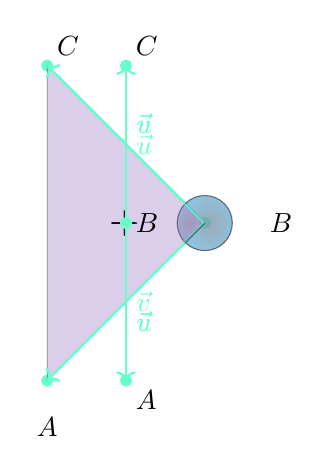
\begin{tikzpicture}
          \coordinate(A) at (0,0);
          \coordinate(B) at (2,2);
          \coordinate(C) at (0,4);
          \coordinate(D) at (-1,2);

          \coordinate(E) at (1,0);
          \coordinate(F) at (1,2);
          \coordinate(G) at (1,4);

          \visible<1-3>{
            \draw[hilight,fill] (A) circle[radius=2pt];
            \draw[hilight,fill] (B) circle[radius=2pt];
            \draw[hilight,fill] (C) circle[radius=2pt];
            \draw (A) node[below=10pt] {$A$};
            \draw (B) node[right=20pt] {$B$};
            \draw (C) node[above right] {$C$};
          }

          \visible<1-2>{
            \draw[thick,hilight,->] (B) -- node[above right] {$\vec v$} (C);
            \draw[thick,hilight,->] (B) -- node[below right] {$\vec u$} (A) ;
          }

          \visible<2>{
            \tkzDrawPolygon[fill=title,opacity=0.3](A,B,C);
            \draw (B) node[left=20pt] {\Large$+$};
            \draw[outer color=title,fill=title,opacity=0.5] (B) -- ++(135:.35cm) arc (135:225:.35cm);
          }

          \visible<3>{
            \tkzDrawPolygon[fill=vhilight,opacity=0.2](A,B,C);
            \draw (B) node[left=20pt] {\Large$-$};
            \draw[thick,hilight,->] (B) -- node[above right] {$\vec u$} (C);
            \draw[thick,hilight,->] (B) -- node[below right] {$\vec v$} (A) ;
            \draw[outer color=title,fill=title,opacity=0.5] (B) -- ++(225:.35cm) arc (225:495:.35cm);
          }

          \visible<4>{
            \draw[thick,hilight,->] (F) -- node[right] {$\vec v$} (E);
            \draw[thick,hilight,->] (F) -- node[right] {$\vec u$} (G) ;
            \draw[hilight,fill] (E) circle[radius=2pt];
            \draw[hilight,fill] (F) circle[radius=2pt];
            \draw[hilight,fill] (G) circle[radius=2pt];
            \draw (E) node[below right] {$A$};
            \draw (F) node[right] {$B$};
            \draw (G) node[above right] {$C$};
          }

        \end{tikzpicture}
      \end{figure}
    \end{column}
    \begin{column}{0.7\textwidth}
      %\footnotesize
      \bi
        \only<1-2>{
          \item Given three points $A$, $B$ and $C$, we want to know if they form
            a counter-clockwise angle in that order.
            \[
              A \rightarrow B \rightarrow C
            \]
          }
        \only<2>{
          \item We can examine the cross product of and the area of the triangle formed by
            \begin{align*}
              \vec{u} = B - C &\quad \vec{v} = B - A \\
              \vec{u} &\times \vec{v} > 0
            \end{align*}
        }

        \only<3->{
          \item The points in the reverse order do not form a counter clockwise angle.
            \[
              C \rightarrow B \rightarrow A
            \]
          \item In the reverse order the vectors swap places
            \begin{align*}
              \vec{u} = B - A &\quad \vec{v} = B - C \\
              \vec{u} &\times \vec{v} < 0
            \end{align*}
        }

        \only<4>{
          \item If the points $A$, $B$ and $C$ are on the same line, then the area will be $0$.
        }
      \ei
    \end{column}
  \end{columns}
\end{frame}

\begin{frame}[fragile]
  \vspace{20pt}
  \begin{minted}{cpp}
double cross(P(a), P(b)) {
    return real(a)*imag(b) - imag(a)*real(x);
}
double ccw(P(a), P(b), P(c)) {
    return cross(b - a, c - b);
}
bool collinear(P(a), P(b), P(c)) {
    return abs(ccw(a, b, c)) < EPS;
}
  \end{minted}
\end{frame}

\subsection{Intersections}
\begin{frame}
  Very common task is to find the intersection of two lines or line segments.
  \bi
    \onslide<2->
    \item Given a pair of points $(x_0, y_0)$, $(x_1, y_1)$, representing a
      line we want to start by obtaining the form $Ax + By = C$.
    \onslide<3->
    \item We can do so by setting
      \begin{align*}
        A &= y_1 - y_0 \\
        B &= x_0 - x_1 \\
        C &= A\cdot x_0 + B\cdot y_1
      \end{align*}
    \onslide<4->
    \vspace{-10pt}
    \item If we have two lines given by such equations, we simply need to solve
      for the two unknowns, $x$ and $y$.
  \ei
\end{frame}

\begin{frame}
  For two lines
  \begin{align*}
    A_0 x + B_0 y = C_0  \\
    A_1 x + B_1 y = C_1
  \end{align*}
  The intersection point is
  \begin{align*}
      x &= \frac{(B_1 \cdot C_0 - B_0 \cdot C_1)}{D} \\
      y &= \frac{(A_0 \cdot C_1 - A_1 \cdot C_0)}{D}
  \end{align*}
  Where
  \[
    D = A_0 \cdot B_1 - A_1 \cdot B_0
  \]
\end{frame}

\begin{frame}[fragile]
  Quite similar problem is to find the intersections of two circles.
  \begin{columns}
    \begin{column}{0.6\textwidth}
      \begin{figure}
        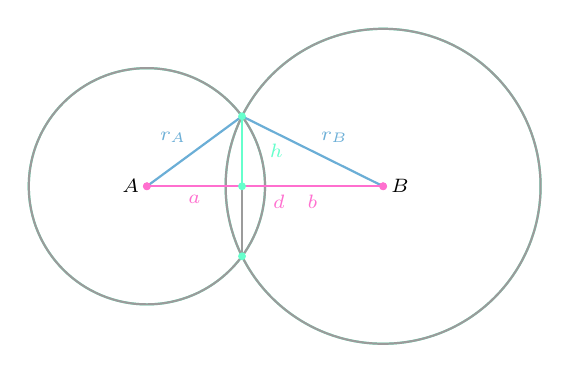
\begin{tikzpicture}[auto,swap]
          \scriptsize
          \coordinate (A) at (0,0);
          \coordinate (B) at (3,0);

          \coordinate (P) at (1.2083333,0);
          \coordinate (Q) at (1.2083333,0.88878037);
          \coordinate (R) at (1.2083333,-0.88878037);

          \draw[title,thick] (A) -- node[above left] {$r_A$} (Q);
          \draw[title,thick] (B) -- node[above right] {$r_B$} (Q);

          \draw (A) node[left] {\scriptsize$A$};
          \draw (B) node[right] {\scriptsize$B$};
          \draw[fill,vhilight] (A) circle[radius=1.2pt];
          \draw[fill,vhilight] (B) circle[radius=1.2pt];
          \draw[hilight,thick] (A) circle[radius=1.5cm];
          \draw[hilight,thick] (B) circle[radius=2cm];

          \visible<1-5>{
            \draw[vhilight,thick] (A) --  node[below,xshift=5pt] {\scriptsize$d$} (B);
          }

          \visible<6->{
            \draw[gray,thick] (A) circle[radius=1.5cm];
            \draw[gray,thick] (B) circle[radius=2cm];
            \draw[fill,vhilight] (A) circle[radius=1.2pt];
            \draw[fill,vhilight] (B) circle[radius=1.2pt];

            \draw[gray,thick] (P) -- (R);
            \draw[hilight,thick] (Q) -- node[right=7pt] {$h$} (P);

            \draw[vhilight, thick] (A) -- node[below] {$a$} (P);
            \draw[vhilight, thick] (B) -- node[below] {$b$} (P);

            \draw[fill,hilight] (P) circle[radius=1.2pt];
            \draw[fill,hilight] (Q) circle[radius=1.2pt];
            \draw[fill,hilight] (R) circle[radius=1.2pt];
          }

        \end{tikzpicture}
      \end{figure}
    \end{column}
    \begin{column}{0.5\textwidth}
      \footnotesize
      \only<2-5>{
        \bi
            \onslide<2-5>{
            \item If $d > r_0 + r_1$ the circles do not intersect.
            }
            \onslide<3-5>{
            \item If $d < \lvert r_0 - r_1 \rvert $, one circles is contained within the other.
            }
            \onslide<4-5>{
            \item If $d = 0$ and $r_0 = r_1$, the circles are the same.
            }
            \onslide<5>{
            \item Let's look at the last case.
            }
        \ei
      }
      \only<6->{
          \bi
            \onslide<6->{
            \item We can solve for the vectors $a$ and $h$ from the equations
                \[
                a^2 + h^2 = r_0^2 \quad b^2 + h^2 = r_1^2
                \]
            }
            \onslide<7->{
            \item We get
                \[
                a = \frac{r_A^2 - r_B^2 + d^2)}{2\cdot d}
                \]
                \[
                h^2 = r_A^2 - a^2
                \]
            }
        \ei
      }
    \end{column}
  \end{columns}
\end{frame}

\begin{frame}[fragile]
  \footnotesize
  \begin{minted}{cpp}
#define C(p, r) const point &p, double r
int intersect(C(A, rA), C(B, rB), point & res1, point & res2) { 
    double d = abs(B - A);
    if ( rA + rB <  d - EPS || d < abs(rA - rB) - EPS){
      return 0;
    }
    double a = (rA*rA - rB*rB + d*d) / 2*d;
    double h = sqrt(rA*rA - a*a);
    point v = normalize(B - A, a);
    u = normalize(rotate(B-A), h);
    res1 = A + v + u;
    res2 = A + v - u;
    if (abs(u) < EPS){
        return 1;
    }
    return 2;
}
  \end{minted}
\end{frame}

\subsection{Polygons}
\begin{frame}
  \begin{columns}
    \begin{column}{0.4\textwidth}
      \begin{figure}
        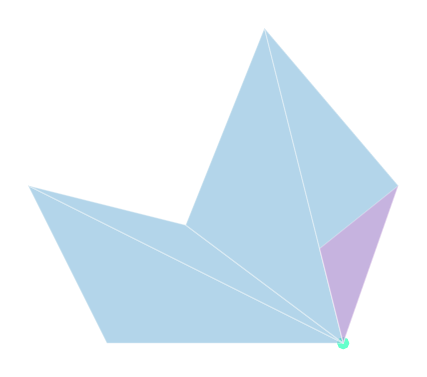
\begin{tikzpicture}
          \coordinate(A) at (0,0);
          \coordinate(B) at (3,0);
          \coordinate(C) at (2.7,1.2);
          \coordinate(D) at (3.7,2);
          \coordinate(E) at (2,4);
          \coordinate(F) at (1,1.5);
          \coordinate(G) at (-1,2);

          \tkzDrawPolygon[color=foreground](A,B,C,D,E,F,G);

          \visible<3->{
            \draw[fill,hilight] (B) circle[radius=2pt];
          }

          \visible<4>{
            \tkzDrawPolygon[color=foreground,fill=title,opacity=0.3,thin](A,B,G);
          }

          \visible<5>{
            \tkzDrawPolygon[color=foreground,fill=title,opacity=0.3,thin](B,G,F);
          }

          \visible<6>{
            \tkzDrawPolygon[color=foreground,fill=title,opacity=0.3,thin](B,F,E);
          }

          \visible<7>{
            \tkzDrawPolygon[color=foreground,fill=title,opacity=0.3,thin](B,E,D);
          }

          \visible<8>{
            \tkzDrawPolygon[color=foreground,fill=vhilight,opacity=0.2,thin](B,D,C);
          }

          \visible<9>{
            \tkzDrawPolygon[color=foreground,fill=title,opacity=0.3,thin](A,B,G);
            \tkzDrawPolygon[color=foreground,fill=title,opacity=0.3,thin](B,G,F);
            \tkzDrawPolygon[color=foreground,fill=title,opacity=0.3,thin](B,F,E);
            \tkzDrawPolygon[color=foreground,fill=title,opacity=0.3,thin](B,E,D);
            \tkzDrawPolygon[color=foreground,fill=vhilight,opacity=0.2,thin](B,D,C);
          }
        \end{tikzpicture}
      \end{figure}
    \end{column}
    \begin{column}{0.6\textwidth}
      \bi
        \item Polygons are represented by a list of points in the order
          representing the edges.
        \onslide<2->
        \item To calculate the area
          \bi
            \onslide<3->
            \item We pick one starting point.
            \onslide<4->
            \item Go through all the other adjacent pair of points and sum the
              area of the triangulation.
            \onslide<8->
            \item Even if we sum up area outside the polygon, due to the cross
              product, it is subtracted later.
          \ei
      \ei
    \end{column}
  \end{columns}
\end{frame}

\begin{frame}[fragile]
  \vspace{20pt}
  %Very simple code.
  \footnotesize
  \begin{minted}{cpp}
double polygon_area_signed(const vector<point> &p) {
    double area = 0;
    int cnt = size(p);
    for (int i = 1; i + 1 < cnt; i++){
        area += cross(p[i] - p[0], p[i + 1] - p[0])/2;
    }
    return area;
}
double polygon_area(vector<point> &p) {
    return abs(polygon_area_signed(p));
}
  \end{minted}
\end{frame}

\subsection{Convex hull}
\begin{frame}[fragile]
  \bi
    \item Given a set of points, we want to find the convex hull of the points.
    \onslide<2->
    \item The convex hull of points can be visualized as the shape formed by a rubber band around the set of points.
  \ei
  \onslide<3->
  \begin{figure}
    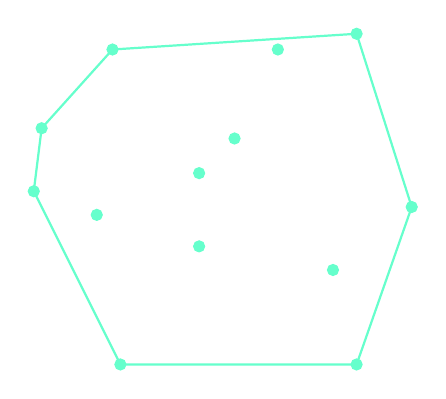
\begin{tikzpicture}
      \coordinate(A) at (0,0);
      \coordinate(B) at (3,0);
      \coordinate(C) at (2.7,1.2);
      \coordinate(D) at (3.7,2);
      \coordinate(E) at (2,4);
      \coordinate(F) at (1,1.5);
      \coordinate(G) at (-1,3);
      \coordinate(H) at (3,4.2);
      \coordinate(I) at (1,2.43);
      \coordinate(J) at (1.45, 2.87);
      \coordinate(K) at (-0.1, 4);
      \coordinate(L) at (-1.1,2.2);
      \coordinate(M) at (-0.3,1.9);

      \draw[fill,hilight] (A) circle[radius=2pt];
      \draw[fill,hilight] (B) circle[radius=2pt];
      \draw[fill,hilight] (C) circle[radius=2pt];
      \draw[fill,hilight] (D) circle[radius=2pt];
      \draw[fill,hilight] (E) circle[radius=2pt];
      \draw[fill,hilight] (F) circle[radius=2pt];
      \draw[fill,hilight] (G) circle[radius=2pt];
      \draw[fill,hilight] (H) circle[radius=2pt];
      \draw[fill,hilight] (I) circle[radius=2pt];
      \draw[fill,hilight] (J) circle[radius=2pt];
      \draw[fill,hilight] (K) circle[radius=2pt];
      \draw[fill,hilight] (L) circle[radius=2pt];
      \draw[fill,hilight] (M) circle[radius=2pt];

      \visible<4->{
        \draw[hilight,thick] (A) -- (B) -- (D) -- (H) -- (K) -- (G) -- (L) -- cycle;
      }
    \end{tikzpicture}
  \end{figure}
\end{frame}

\begin{frame}[fragile]
  \vspace{20pt}
  Graham scan:
  \bi
    \onslide<2->
    \item Pick the point $p_0$ with the lowest $y$ coordinate.
    \onslide<3->
    \item Sort all the points by polar angle with $p_0$.
    \onslide<4->
    \item Iterate through all the points
    \onslide<5->
    \item If the current point forms a clockwise angle with the last two
      points, remove last point from the convex set.
    \onslide<6->
    \item Otherwise, add the current point to the convex set.
  \ei
  \onslide<7->
  Time complexity $O(N \log N)$.
\end{frame}

\begin{frame}
  \begin{figure}
    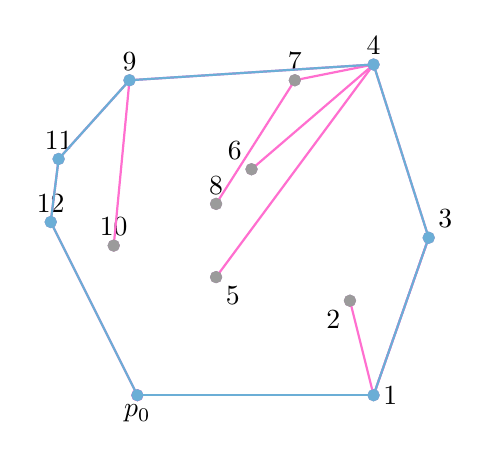
\begin{tikzpicture}
      \coordinate(A) at (0,0);
      \coordinate(B) at (3,0);
      \coordinate(C) at (2.7,1.2);
      \coordinate(D) at (3.7,2);
      \coordinate(E) at (2,4);
      \coordinate(F) at (1,1.5);
      \coordinate(G) at (-1,3);
      \coordinate(H) at (3,4.2);
      \coordinate(I) at (1,2.43);
      \coordinate(J) at (1.45, 2.87);
      \coordinate(K) at (-0.1, 4);
      \coordinate(L) at (-1.1,2.2);
      \coordinate(M) at (-0.3,1.9);

      %\draw[fill,hilight] (A) circle[radius=2pt];
      \onslide<2->{
        \draw[fill,hilight] (B) circle[radius=2pt];
        \draw[fill,hilight] (C) circle[radius=2pt];
        \draw[fill,hilight] (D) circle[radius=2pt];
        \draw[fill,hilight] (E) circle[radius=2pt];
        \draw[fill,hilight] (F) circle[radius=2pt];
        \draw[fill,hilight] (G) circle[radius=2pt];
        \draw[fill,hilight] (H) circle[radius=2pt];
        \draw[fill,hilight] (I) circle[radius=2pt];
        \draw[fill,hilight] (J) circle[radius=2pt];
        \draw[fill,hilight] (K) circle[radius=2pt];
        \draw[fill,hilight] (L) circle[radius=2pt];
        \draw[fill,hilight] (M) circle[radius=2pt];
        \draw[fill,vhilight] (A) circle[radius=2pt];
      }

      \visible<3-4>{
        \draw[very thin,foreground] (A) -- (B);
        \draw[very thin,foreground] (A) -- (C);
        \draw[very thin,foreground] (A) -- (D);
        \draw[very thin,foreground] (A) -- (E);
        \draw[very thin,foreground] (A) -- (F);
        \draw[very thin,foreground] (A) -- (G);
        \draw[very thin,foreground] (A) -- (H);
        \draw[very thin,foreground] (A) -- (I);
        \draw[very thin,foreground] (A) -- (J);
        \draw[very thin,foreground] (A) -- (K);
        \draw[very thin,foreground] (A) -- (L);
        \draw[very thin,foreground] (A) -- (M);
      }

      \visible<4->{
        \draw (A) node[below] {$p_0$};
        \draw (B) node[right] {$1$};
        \draw (C) node[below left] {$2$};
        \draw (D) node[above right] {$3$};
        \draw (E) node[above] {$7$};
        \draw (F) node[below right] {$5$};
        \draw (G) node[above] {$11$};
        \draw (H) node[above] {$4$};
        \draw (I) node[above] {$8$};
        \draw (J) node[above left] {$6$};
        \draw (K) node[above] {$9$};
        \draw (L) node[above] {$12$};
        \draw (M) node[above] {$10$};
      }

      \visible<5->{
        \draw[fill,vhilight] (B) circle[radius=2pt];

      }
      \visible<5-7>{
        \draw[fill,vhilight] (C) circle[radius=2pt];
      }
      \visible<5>{
        \draw[thick, vhilight] (B) -- (C);
      }
      \visible<5->{
        \draw[thick, vhilight] (A) -- (B);
      }
      \visible<6->{
        \draw[fill,gray] (C) circle[radius=2pt];
      }
      \visible<6->{
        \draw[fill,vhilight] (D) circle[radius=2pt];
      }
      \visible<6->{
        \draw[thick, vhilight] (B) -- (D);
      }
      %\visible<7->{
        %\draw[fill,title] (A) circle[radius=2pt];
        %\draw[thick, title] (A) -- (B);
      %}
      \visible<7>{
        \draw[thick, vhilight] (B) -- (D);
      }
      %\visible<8->{
        %\draw[fill,title] (B) circle[radius=2pt];
        %\draw[thick, title] (B) -- (D);
      %}
      \visible<7->{
        \draw[thick, vhilight] (D) -- (H);
      }
      \visible<7->{
        \draw[fill,vhilight] (H) circle[radius=2pt];
      }
      \visible<8>{
        \draw[thick, vhilight] (H) -- (F);
        \draw[fill,vhilight] (F) circle[radius=2pt];
      }
      \visible<9->{
        \draw[fill,gray] (F) circle[radius=2pt];
      }
      \visible<9>{
        \draw[thick, vhilight] (H) -- (J);
        \draw[fill,vhilight] (J) circle[radius=2pt];
      }
      \visible<10->{
        \draw[fill,gray] (J) circle[radius=2pt];
      }
      \visible<10-11>{
        \draw[thick, vhilight] (H) -- (E);
        \draw[fill,vhilight] (E) circle[radius=2pt];
      }
      %\visible<11-12>{
        %\draw[fill,gray] (E) circle[radius=2pt];
      %}
      \visible<11>{
        \draw[thick, vhilight] (E) -- (I);
        \draw[fill,vhilight] (I) circle[radius=2pt];
      }

      \visible<12->{
        \draw[fill,gray] (E) circle[radius=2pt];
        \draw[fill,gray] (I) circle[radius=2pt];
      }
      \visible<12->{
        \draw[thick, vhilight] (H) -- (K);
      }
      \visible<12->{
        \draw[fill,vhilight] (K) circle[radius=2pt];
      }
      %\visible<13->{
        %\draw[thick, title] (D) -- (H);
        %\draw[fill,title] (D) circle[radius=2pt];
      %}
      \visible<13>{
        \draw[thick, vhilight] (K) -- (M);
        \draw[fill,vhilight] (M) circle[radius=2pt];
      }
      \visible<14->{
        \draw[fill,gray] (M) circle[radius=2pt];
      }
      \visible<14->{
        \draw[thick, vhilight] (K) -- (G);
      }
      \visible<14->{
        \draw[fill,vhilight] (G) circle[radius=2pt];
      }
      %\visible<15->{
        %\draw[fill,title] (H) circle[radius=2pt];
        %\draw[thick, title] (H) -- (K);
      %}
      \visible<15->{
        \draw[thick, vhilight] (G) -- (L);
        \draw[fill,vhilight] (L) circle[radius=2pt];
      }
      %\visible<16->{
        %\draw[fill,title] (K) circle[radius=2pt];
        %\draw[thick, title] (K) -- (G);
      %}
      \visible<16>{
        \draw[thick, vhilight] (L) -- (A);
        \draw[fill,vhilight] (A) circle[radius=2pt];
      }
      \visible<17->{
        \draw[thick, title] (A) -- (B);
        \draw[thick, title] (B) -- (D);
        \draw[thick, title] (D) -- (H);
        \draw[thick, title] (H) -- (K);
        \draw[thick, title] (K) -- (G);
        \draw[thick, title] (G) -- (L);
        \draw[thick, title] (L) -- (A);
        \draw[fill,title] (A) circle[radius=2pt];
        \draw[fill,title] (B) circle[radius=2pt];
        \draw[fill,title] (D) circle[radius=2pt];
        \draw[fill,title] (H) circle[radius=2pt];
        \draw[fill,title] (K) circle[radius=2pt];
        \draw[fill,title] (G) circle[radius=2pt];
        \draw[fill,title] (L) circle[radius=2pt];
      }

    \end{tikzpicture}
  \end{figure}
\end{frame}

\begin{frame}[fragile]
  \scriptsize
  \begin{minted}{cpp}
point hull[MAXN];
int convex_hull(vector<point> p) {
    int n = size(p), l = 0;
    sort(p.begin(), p.end(), cmp);
    for (int i = 0; i < n; i++) {
        if (i > 0 && p[i] == p[i - 1]) 
            continue;
        while (l >= 2 && ccw(hull[l - 2], hull[l - 1], p[i]) >= 0)
            l--;
        hull[l++] = p[i];
    }
    int r = l;
    for (int i = n - 2; i >= 0; i--) {
        if (p[i] == p[i + 1])
            continue;
        while (r - l >= 1 && ccw(hull[r - 2], hull[r - 1], p[i]) >= 0)
            r--;
        hull[r++] = p[i];
    }
    return l == 1 ? 1 : r - 1;
}
  \end{minted}
\end{frame}

\begin{frame}
  \vspace{40pt}
  Many other algorithms exist
  \bi
    \onslide<2->
    \item Gift wrapping aka Jarvis march.
    \onslide<3->
    \item Quick hull, similar idea to quicksort.
    \onslide<4->
    \item Divide and conquer.
  \ei
  \onslide<5->
  Some can be extended to three dimensions, or higher.
\end{frame}

\subsection{Point in convex polygon}
\begin{frame}
  Simple algorithm to check if a point is in a convex polygon.
  \begin{columns}
    \begin{column}{0.6\textwidth}
      \begin{figure}
        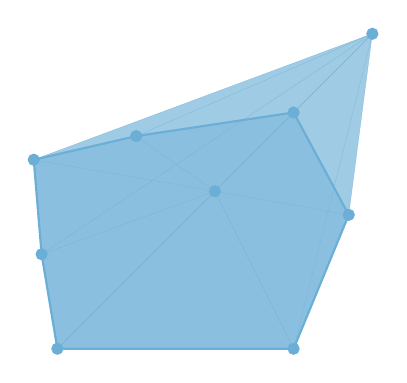
\begin{tikzpicture}
          \coordinate(A) at (0,0);
          \coordinate(B) at (3,0);
          \coordinate(C) at (3.7,1.7);
          \coordinate(D) at (3,3);
          \coordinate(E) at (1, 2.7);
          \coordinate(F) at (-0.3,2.4);
          \coordinate(G) at (-0.2,1.2);

          \coordinate(P) at (4,4);
          \coordinate(Q) at (2,2);

          \draw[fill,title] (A) circle[radius=2pt];
          \draw[fill,title] (B) circle[radius=2pt];
          \draw[fill,title] (C) circle[radius=2pt];
          \draw[fill,title] (D) circle[radius=2pt];
          \draw[fill,title] (E) circle[radius=2pt];
          \draw[fill,title] (F) circle[radius=2pt];
          \draw[fill,title] (G) circle[radius=2pt];

          \visible<1-10>{
            \draw[fill,title] (P) circle[radius=2pt];
          }

          \visible<11->{
            \draw[fill,title] (Q) circle[radius=2pt];
          }

          \draw[title,thick] (A) -- (B) -- (C) -- (D) -- (E) -- (F) -- (G) -- cycle;
          \visible<2>{
            \tkzDrawPolygon[color=title,fill=title,opacity=0.4,ultra thin](A,B,C,D,E,F,G);
          }
          \visible<3-10>{
            \tkzDrawPolygon[color=title,fill=title,opacity=0.4,ultra thin](A,B,P);
          }
          \visible<4-10>{
            \tkzDrawPolygon[color=title,fill=title,opacity=0.4,ultra thin](B,C,P);
          }
          \visible<5-10>{
            \tkzDrawPolygon[color=title,fill=title,opacity=0.4,ultra thin](C,D,P);
          }
          \visible<6-10>{
            \tkzDrawPolygon[color=title,fill=title,opacity=0.4,ultra thin](D,E,P);
          }
          \visible<7-10>{
            \tkzDrawPolygon[color=title,fill=title,opacity=0.4,ultra thin](E,F,P);
          }
          \visible<8-10>{
            \tkzDrawPolygon[color=title,fill=title,opacity=0.4,ultra thin](F,G,P);
          }
          \visible<9-10>{
            \tkzDrawPolygon[color=title,fill=title,opacity=0.4,ultra thin](G,A,P);
          }

          \visible<11->{
            \tkzDrawPolygon[color=title,fill=title,opacity=0.4,ultra thin](A,B,Q);
          }
          \visible<12->{
            \tkzDrawPolygon[color=title,fill=title,opacity=0.4,ultra thin](B,C,Q);
          }
          \visible<13->{
            \tkzDrawPolygon[color=title,fill=title,opacity=0.4,ultra thin](C,D,Q);
          }
          \visible<14->{
            \tkzDrawPolygon[color=title,fill=title,opacity=0.4,ultra thin](D,E,Q);
          }
          \visible<15->{
            \tkzDrawPolygon[color=title,fill=title,opacity=0.4,ultra thin](E,F,Q);
          }
          \visible<16->{
            \tkzDrawPolygon[color=title,fill=title,opacity=0.4,ultra thin](F,G,Q);
          }
          \visible<17->{
            \tkzDrawPolygon[color=title,fill=title,opacity=0.4,ultra thin](G,A,Q);
          }

        \end{tikzpicture}
      \end{figure}
    \end{column}
    \begin{column}{0.5\textwidth}
      \footnotesize
      \bi
        \onslide<2->
        \item We start by calculating the area of the polygon.
        \onslide<3->
        \item To check if our point is contained in the polygon we sum up the
          area of the triangles formed the point and every two adjacent points.
        \onslide<10->
        \item The total area of the triangles is equal to the area of the
          polygon iff the point is inside the polygon.
      \ei
    \end{column}
  \end{columns}
\end{frame}

\subsection{Point in concave polygon}
\begin{frame}
  \vspace{40pt}
  How about non convex polygon?
  \bi
    \onslide<2->
    \item The \emph{even-odd rule} algorithm.
    \onslide<3->
    \item We examine a ray passing through the polygon to the point.
    \onslide<4->
    \item If the ray crosses the boundary of the polygon, then it alternately
      goes from outside to inside, and outside to inside.
  \ei
\end{frame}

\begin{frame}
  \begin{columns}
    \begin{column}{0.6\textwidth}
      \begin{figure}
        \begin{tikzpicture}
            \coordinate(A) at (0,0);
            \coordinate(B) at (3.5,0);
            \coordinate(C) at (2.7,1.2);
            \coordinate(D) at (4.2,3);
            \coordinate(E) at (2.5,1.3);
            \coordinate(F) at (1.7,4);
            \coordinate(G) at (0.8,1.2);
            \coordinate(H) at (-1,2.5);

            \coordinate(P) at (-1.7,1.7);
            \coordinate(Q) at (5,1.7);

            \coordinate(R) at (1,4);
            \coordinate(S) at (0.3, 2);

            \coordinate(O) at (3.4, 1.7);
            \onslide<1-2>{
              \draw[fill,hilight] (O) circle[radius=2pt];
            }

            \tkzInterLL(B,D)(P,Q) \tkzGetPoint{LL1};
            \tkzInterLL(D,E)(P,Q) \tkzGetPoint{LL2};
            \tkzInterLL(E,F)(P,Q) \tkzGetPoint{LL3};
            \tkzInterLL(F,G)(P,Q) \tkzGetPoint{LL4};
            \tkzInterLL(G,H)(P,Q) \tkzGetPoint{LL5};
            \tkzInterLL(H,A)(P,Q) \tkzGetPoint{LL6};

            \tkzInterLL(D,E)(R,O) \tkzGetPoint{LL7};
            \tkzInterLL(E,F)(R,O) \tkzGetPoint{LL8};
            \tkzInterLL(F,G)(R,O) \tkzGetPoint{LL9};

            \tkzInterLL(B,D)(S,Q) \tkzGetPoint{LL10};
            \tkzInterLL(D,E)(S,Q) \tkzGetPoint{LL11};
            \tkzInterLL(E,F)(S,Q) \tkzGetPoint{LL12};
            \tkzInterLL(F,G)(S,Q) \tkzGetPoint{LL13};

            \tkzDrawPolygon[color=foreground,opacity=0.85](A,B,D,E,F,G,H);

            \onslide<2-4>{
              %\tkzDrawPolygon[color=foreground,opacity=0.7](A,B,D,E,F,G,H);
              \draw[vhilight,title] (P) -- (O);
              \draw[fill,hilight] (O) circle[radius=2pt];
            }

            \onslide<3-4>{
              \draw[fill,vhilight] (LL2) circle[radius=2pt];
              \draw[fill,vhilight] (LL3) circle[radius=2pt];
              \draw[fill,vhilight] (LL4) circle[radius=2pt];
              \draw[fill,vhilight] (LL5) circle[radius=2pt];
              \draw[fill,vhilight] (LL6) circle[radius=2pt];
            }

            \onslide<5-6>{
              \draw[vhilight,title] (R) -- (O);
              \draw[fill,hilight] (O) circle[radius=2pt];
            }

            \onslide<6>{
              \draw[fill,vhilight] (LL7) circle[radius=2pt];
              \draw[fill,vhilight] (LL8) circle[radius=2pt];
              \draw[fill,vhilight] (LL9) circle[radius=2pt];
            }

            \onslide<7-8>{
              %\tkzDrawPolygon[color=foreground,opacity=0.7](A,B,D,E,F,G,H);
              \draw[vhilight,title] (Q) -- (S);
              \draw[fill,hilight] (S) circle[radius=2pt];
            }

            \onslide<8>{
              \draw[fill,vhilight] (LL10) circle[radius=2pt];
              \draw[fill,vhilight] (LL11) circle[radius=2pt];
              \draw[fill,vhilight] (LL12) circle[radius=2pt];
              \draw[fill,vhilight] (LL13) circle[radius=2pt];
            }

        \end{tikzpicture}
      \end{figure}
    \end{column}
    \begin{column}{0.5\textwidth}
      \bi
        \onslide<2->
        \item Ray from the outside of the polygon to the point.
        \onslide<3->
        \item Count the number of intersection points.
        \onslide<4->
        \item If odd, then the point is inside the polygon.
        \item If even, then the point is outside the polygon.
        \onslide<5->
        \item Does not matter which ray we pick.
      \ei
    \end{column}
  \end{columns}
\end{frame}

\subsection{Closest pair of points}
\begin{frame}
  \vspace{20pt}
  Given a set of points, we want to find the pair of points with the smallest distance between them. \\
  \vspace{5pt}
  Divide and conquer algorithm;
  \bi
    \onslide<2->
    \item Sort points by the $x$-coordinate.
    \onslide<3->
    \item Split the set into two equal sized sets by the vertical line of the medial $x$ value.
    \onslide<4->
    \item Solve the problem recursively in the left and right subset.
    \onslide<5->
    \item Sort the two subsets by the $y$-coordinate.
    \onslide<6->
    \item Find the smallest distance among the pair of points which lie on different sides of the line.
  \ei
\end{frame}

\begin{frame}{}
  \vspace{30pt}
  Takk fyrir önnina! \\
  \vspace{15pt}
  Gangi ykkur vel og góða skemmtun í prófinu á morgun!
\end{frame}

% TODO: MAYBE Floating point IF NOT COVERED
% TODO: Point representation
% TODO: Line representation
% TODO: Line segment representation
% TODO: Circles
%  - Geometric properties, circumference, area
% TODO: Triangles
%  - Area of a triangle
%  - Point in triangle
% TODO: Rectangles
% TODO: Distance between geometric objects, line-line, point-line
% TODO: Intersections of geometric objects, mainly lines and line segments
% TODO: MAYBE Spheres
% TODO: CCW
% TODO: Polygon
% TODO: Representation of polygon
% TODO: Polygon area
% TODO: Point in Polygon
% TODO: Convexity
% TODO: Convex hull
% TODO: Divide & Conquer
% TODO: Closest pair of points
%
\end{document}

